\section{Exercise 2}
\subsection{Problem 1: Gershgorin Disks}
\[
    A = \begin{bmatrix}
        -2  & 1    & 0   \\
        1   & 3    & 0.5 \\
        0.5 & -0.5 & 4
    \end{bmatrix},
    \quad
    B = \begin{bmatrix}
        2  & -1 & 0  \\
        -1 & 2  & -1 \\
        0  & -1 & 1
    \end{bmatrix},
    \quad
    C = \begin{bmatrix}
        1     & 0.5i  & 0.5i   \\
        0.5   & i     & 0.5    \\
        -0.5i & -0.5i & 1 + 2i
    \end{bmatrix}
\]
Compute centers and radii (row-form Gershgorin):

\begin{minipage}{0.5\textwidth}
    For \(A\):
    \begin{align*}
        a_{11} & = -2, \quad r_1 = |1| + |0| = 1 & \Rightarrow & D(-2,1)  \\
        a_{22} & = 3, \quad r_2 = |1| + |0.5| = 1.5 & \Rightarrow & D(3,1.5) \\
        a_{33} & = 4, \quad r_3 = |0.5| + |-0.5| = 1 & \Rightarrow & D(4,1)
    \end{align*}
    Eigenvalues:
    \begin{align*}
        \lambda_1 &\in D(-2,1)\\
        \lambda_{2,3} &\in D(3,1.5) \cup D(4,1)
    \end{align*}
\end{minipage}%
\begin{minipage}{0.5\textwidth}
    \begin{center}
        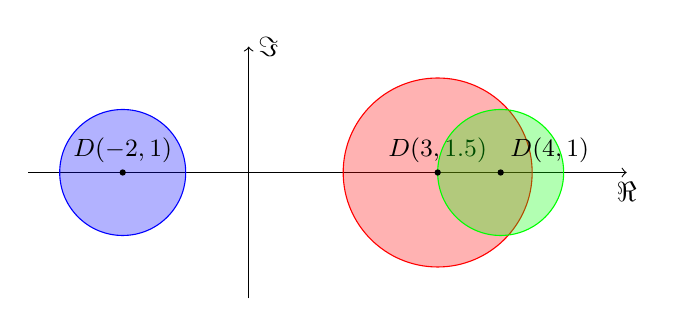
\begin{tikzpicture}[scale=0.8]
            % axes
            \draw[->] (-3.5,0) -- (6,0) node[below] {$\Re$};
            \draw[->] (0,-2) -- (0,2) node[right] {$\Im$};
            % disks with transparent fill
            \draw[fill=blue, fill opacity=0.3, draw=blue] (-2,0) circle (1) node[above, font=\small, fill opacity=1] {$D(-2,1)$};
            \draw[fill=red, fill opacity=0.3, draw=red] (3,0) circle (1.5) node[above, font=\small, fill opacity=1] {$D(3,1.5)$};
            \draw[fill=green, fill opacity=0.3, draw=green] (4,0) circle (1) node[above right, font=\small, fill opacity=1] {$D(4,1)$};
            % center markers
            \fill (-2,0) circle (0.05);
            \fill (3,0) circle (0.05);
            \fill (4,0) circle (0.05);
        \end{tikzpicture}
    \end{center}
\end{minipage}
\begin{minipage}{0.6\textwidth}
    For \(B\):
    \begin{align*}
        b_{11} & = 2, \quad s_1 = |-1| + |0| = 1 & \Rightarrow & D(2,1) \\
        b_{22} & = 2, \quad s_2 = |-1| + |-1| = 2 & \Rightarrow & D(2,2) \\
        b_{33} & = 1, \quad s_3 = |0| + |-1| = 1 & \Rightarrow & D(1,1)
    \end{align*}
    Eigenvalues:
    \begin{align*}
        \lambda_{1,2,3} &\in D(2,2)
    \end{align*}
\end{minipage}%
\begin{minipage}{0.4\textwidth}
    \begin{center}
        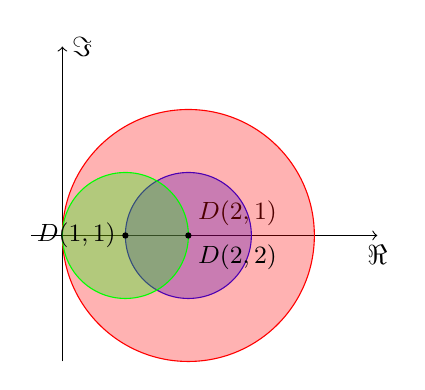
\begin{tikzpicture}[scale=0.8]
            \draw[->] (-0.5,0) -- (5,0) node[below] {$\Re$};
            \draw[->] (0,-2) -- (0,3) node[right] {$\Im$};
            % disks with transparent fill
            \draw[fill=blue, fill opacity=0.3, draw=blue] (2,0) circle (1) node[above right, font=\small, fill opacity=1] {$D(2,1)$};
            \draw[fill=red, fill opacity=0.3, draw=red] (2,0) circle (2) node[below right, font=\small, fill opacity=1] {$D(2,2)$};
            \draw[fill=green, fill opacity=0.3, draw=green] (1,0) circle (1) node[left, font=\small, fill opacity=1] {$D(1,1)$};
            % center markers
            \fill (2,0) circle (0.05);
            \fill (1,0) circle (0.05);
        \end{tikzpicture}
    \end{center}
\end{minipage}

\begin{minipage}{0.6\textwidth}
    For \(C\) (centers are complex; plot in complex plane):
    \begin{align*}
        c_{11} & = 1, \quad t_1 = |0.5i| + |0.5i| = 1 & \Rightarrow & D(1,1)    \\
        c_{22} & = i, \quad t_2 = |0.5| + |0.5| = 1 & \Rightarrow & D(i,1)    \\
        c_{33} & = 1+2i, \quad t_3 = |-0.5i| + |-0.5i| = 1 & \Rightarrow & D(1+2i,1)
    \end{align*}
    Eigenvalues:
    \begin{align*}
        \lambda_{1,2,3} &\in D(1,1) \cup D(i,1) \cup D(1+2i,1)
    \end{align*}
\end{minipage}%
\begin{minipage}{0.4\textwidth}
    \begin{center}
        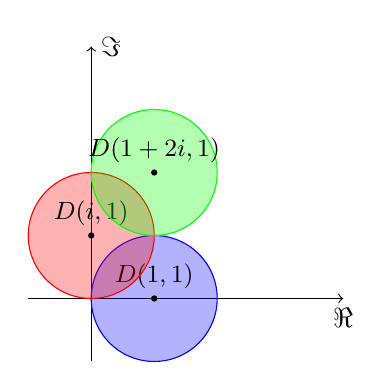
\begin{tikzpicture}[scale=0.8]
            \draw[->] (-1,0) -- (4,0) node[below] {$\Re$};
            \draw[->] (0,-1) -- (0,4) node[right] {$\Im$};
            % disks with transparent fill (centers: (1,0), (0,1), (1,2))
            \draw[fill=blue, fill opacity=0.3, draw=blue] (1,0) circle (1) node[above, font=\small, fill opacity=1] {$D(1,1)$};
            \draw[fill=red, fill opacity=0.3, draw=red] (0,1) circle (1) node[above, font=\small, fill opacity=1] {$D(i,1)$};
            \draw[fill=green, fill opacity=0.3, draw=green] (1,2) circle (1) node[above, font=\small, fill opacity=1] {$D(1+2i,1)$};
            % center markers
            \fill (1,0) circle (0.05);
            \fill (0,1) circle (0.05);
            \fill (1,2) circle (0.05);
        \end{tikzpicture}
    \end{center}
\end{minipage}
